\begin{landscape}
  \begin{table}[!htb]
    \caption{Facetas do pensamento computacional extraídos de material voltado para implementação do pensamento educacional nas escolas}
    \label{tab:facetas}
    \footnotesize
    \center  
    \begin{tabular}{L{5cm}L{6cm}L{5cm}L{5cm}}
      \hline
      Atividade & Faceta & Prática Envolvida & Classificação taxonômica da prática \\
      \hline
      \\
      \multirow{3}{*}{\shortstack[l]{Projeto de construtor de\\ montanha-russa\\ \\ 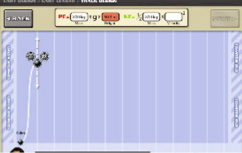
\includegraphics[width=4.0cm]{imagens/rollerecoster.png}}} & Os alunos constroem modelos de montanhas-russas que podem ser executadas, gerando dados sobre a energia da montanha-russa  & Obter insight / compreensão de simulações / modelos baseados em computador & Uso de um modelo computacional para entender um conceito \\ 
      &&& Construção de modelos computacionais. \\
      \\
      & Os alunos registram medições de energia em quatro pontos da pista e armazenam os dados em uma tabela & Fazer medições efetivas a partir de uma simulação & Coleta de dados \\\\ \cline{1-4}
      \\
      \multirow{4}{*}{\shortstack[l]{Desenho de uma\\ montanha-russa\\ \\ 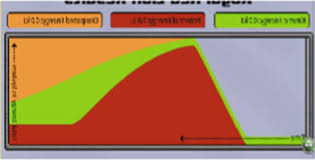
\includegraphics[width=4.0cm]{imagens/roller-coster-kinectic.jpeg} \\\\ Gráfico das energias \\ cinéticas e potenciais\\ da montanha-russa\\ ao longo do tempo}} & São necessárias várias iterações para construir uma montanha russa de sucesso que termine a pista e não trave & Abordagem iterativa para a construção de uma solução & Uso de modelos computacionais para encontrar e testar uma solução \\ 
      \\
      &&& Investigação sistemática das causas de um problema (\textit{troubleshooting}) e depuração (\textit{debugging}) \\
     \\ 
      & Traduzindo em gráficos de tela de energia potencial / cinética em forma de tabela & Mensurar a adequação de uma representação avaliando seus pontos fortes e fracos. & Manipulação de dados \\
      &&& Visualização de dados \\\\ \cline{1-4}
    \end{tabular}
  \end{table}
  \legend{Fonte: Adaptado de \citeonline{Weintrop2016}}
\end{landscape}
